\renewcommand{\arraystretch}{0}
\begin{figure*}[ht]
\centering
\begin{tabular}{cc}
%[trim=left bottom right top, clip]
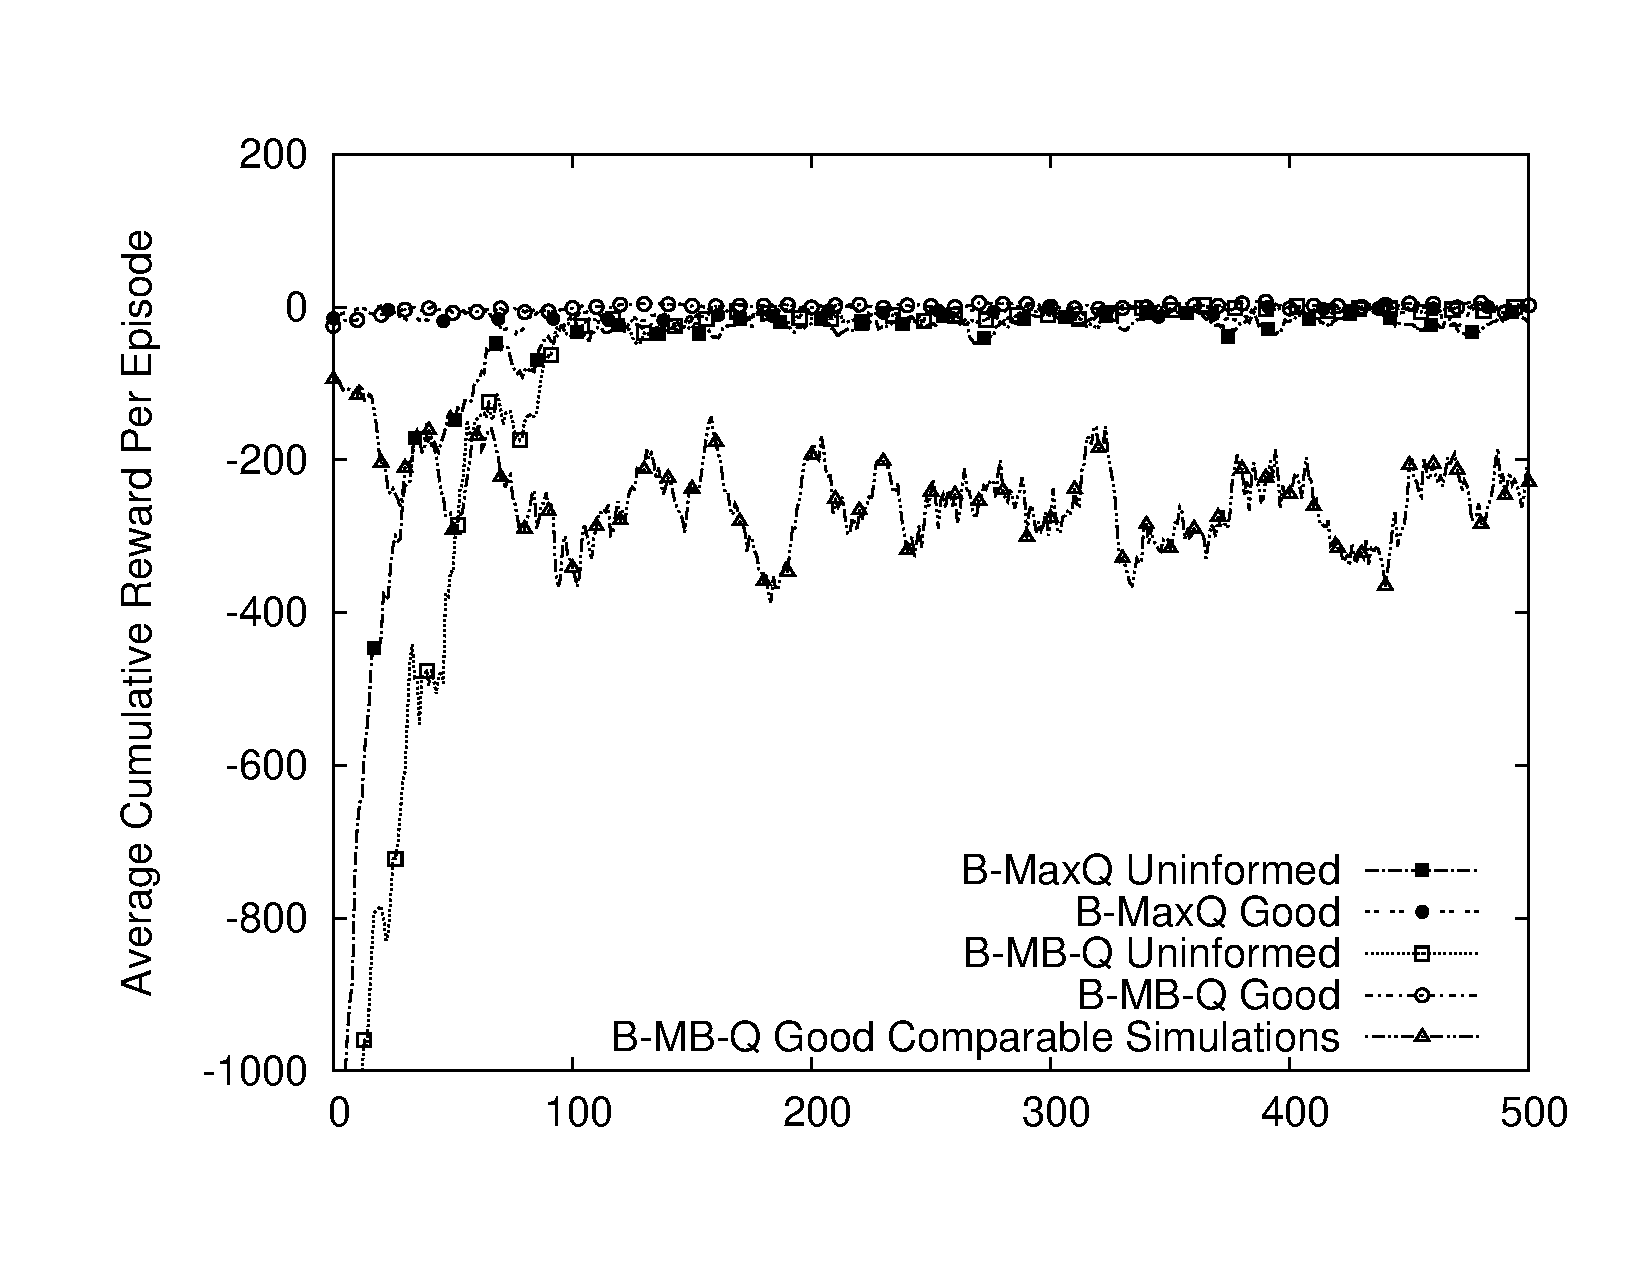
\includegraphics[trim=50 50 30 50, clip, scale=0.3]{exp/Taxib.pdf} & 
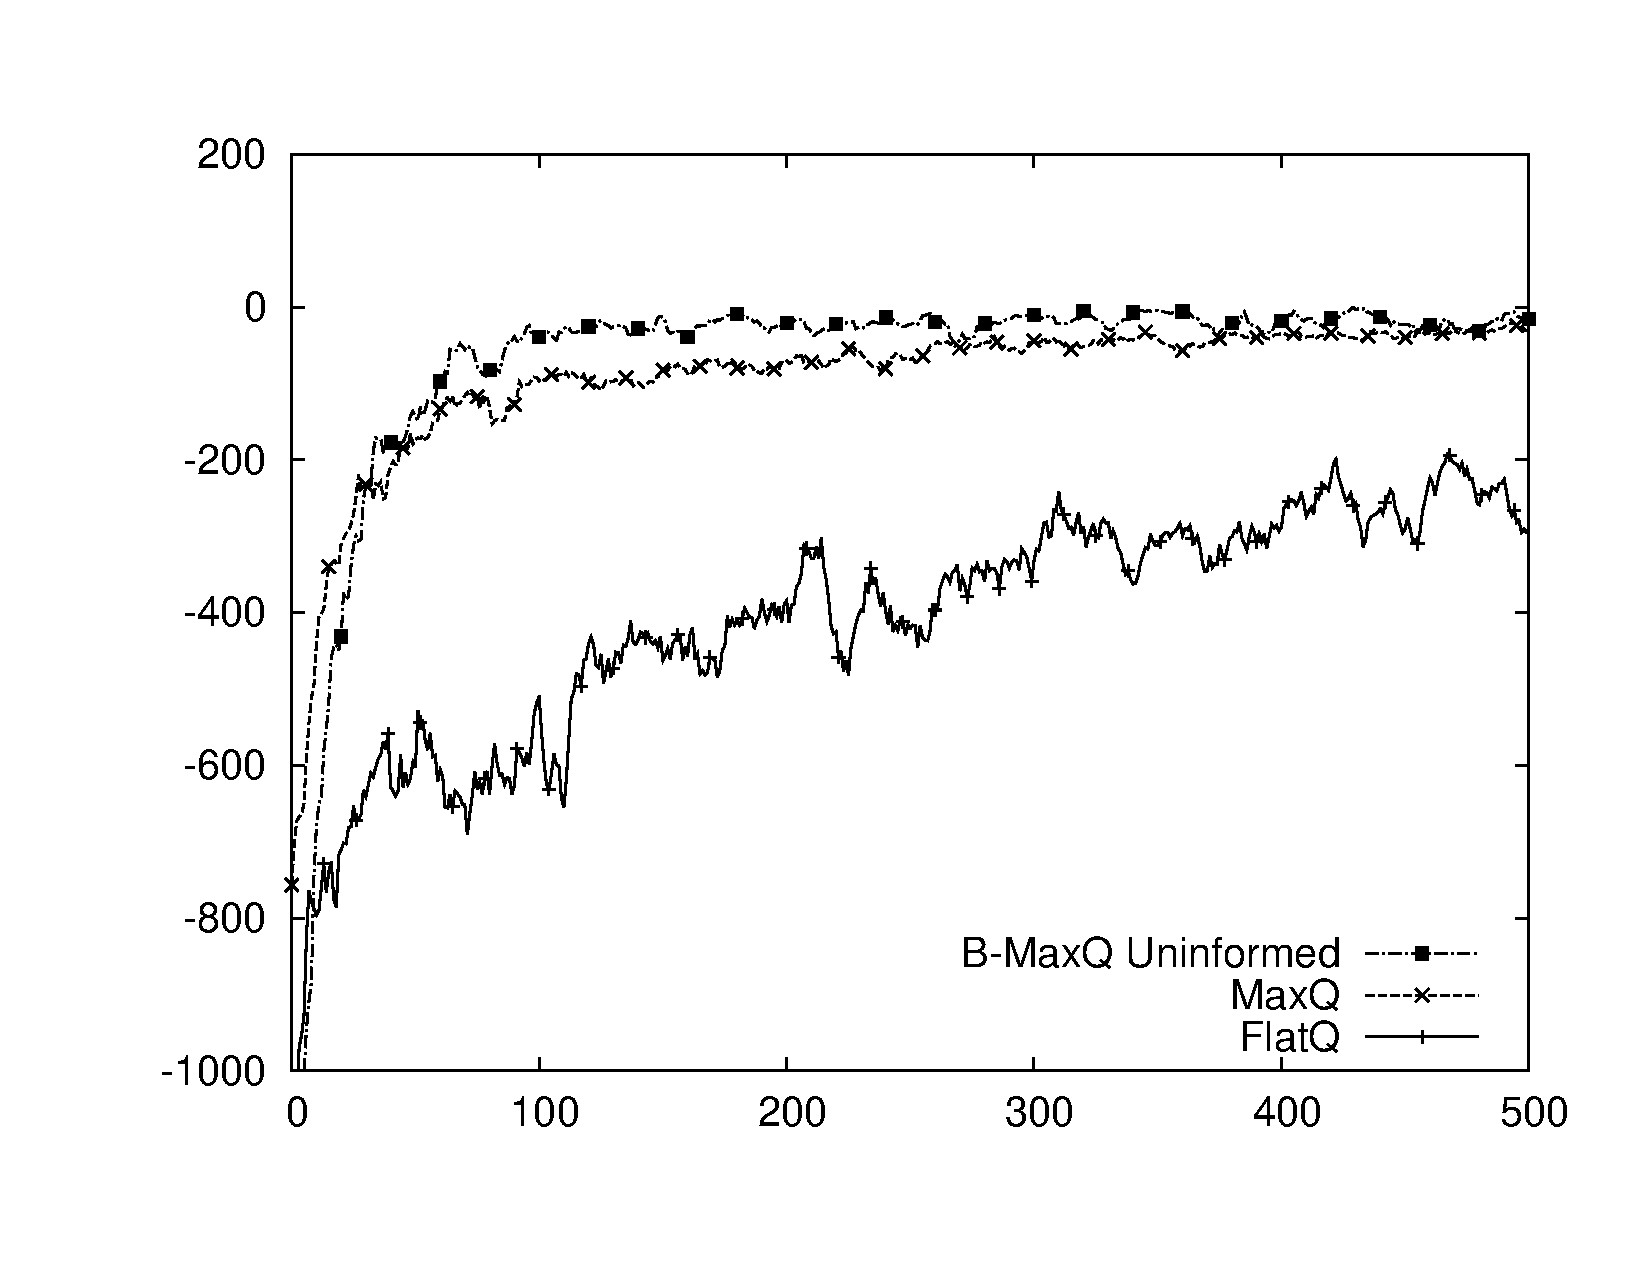
\includegraphics[trim=50 50 30 50, clip, scale=0.3]{exp/Taxinb.pdf} \\
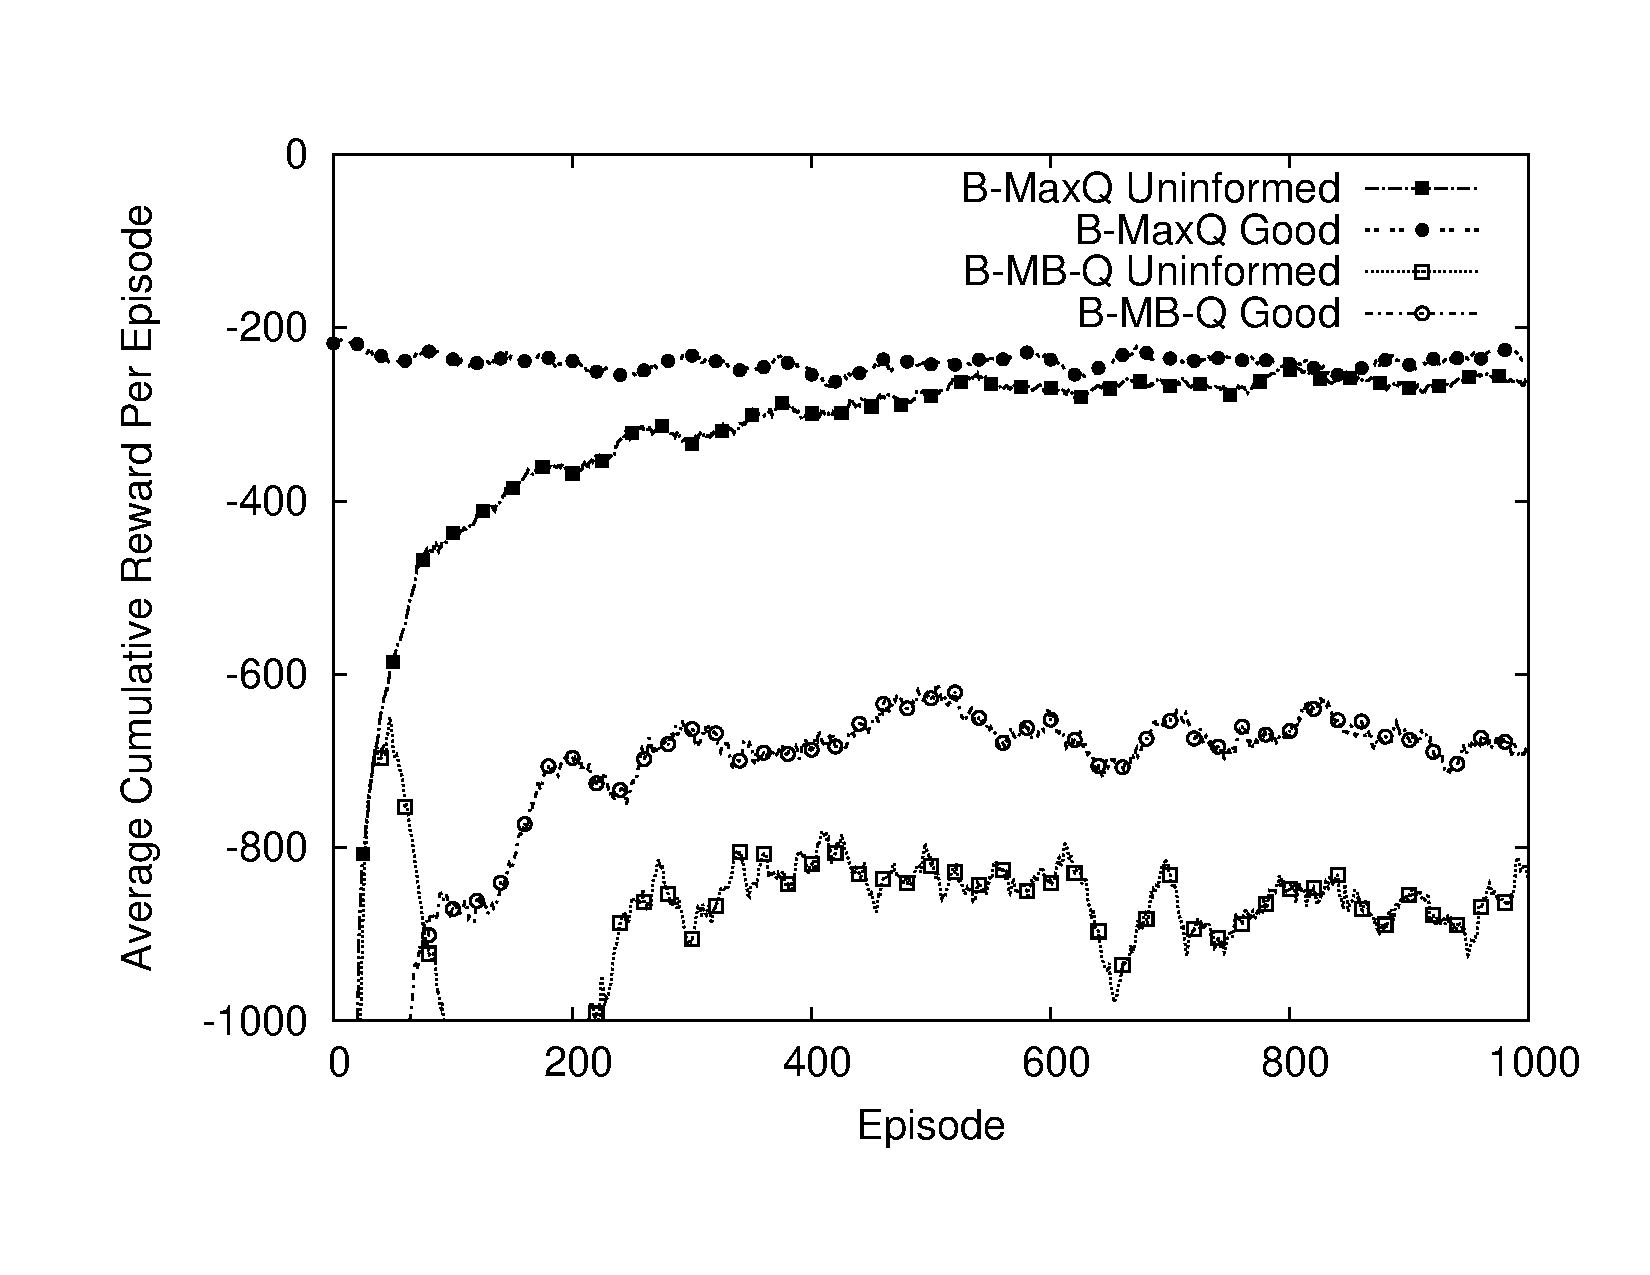
\includegraphics[trim=50 50 30 50, clip, scale=0.3]{exp/Wargus3322b.pdf} & 
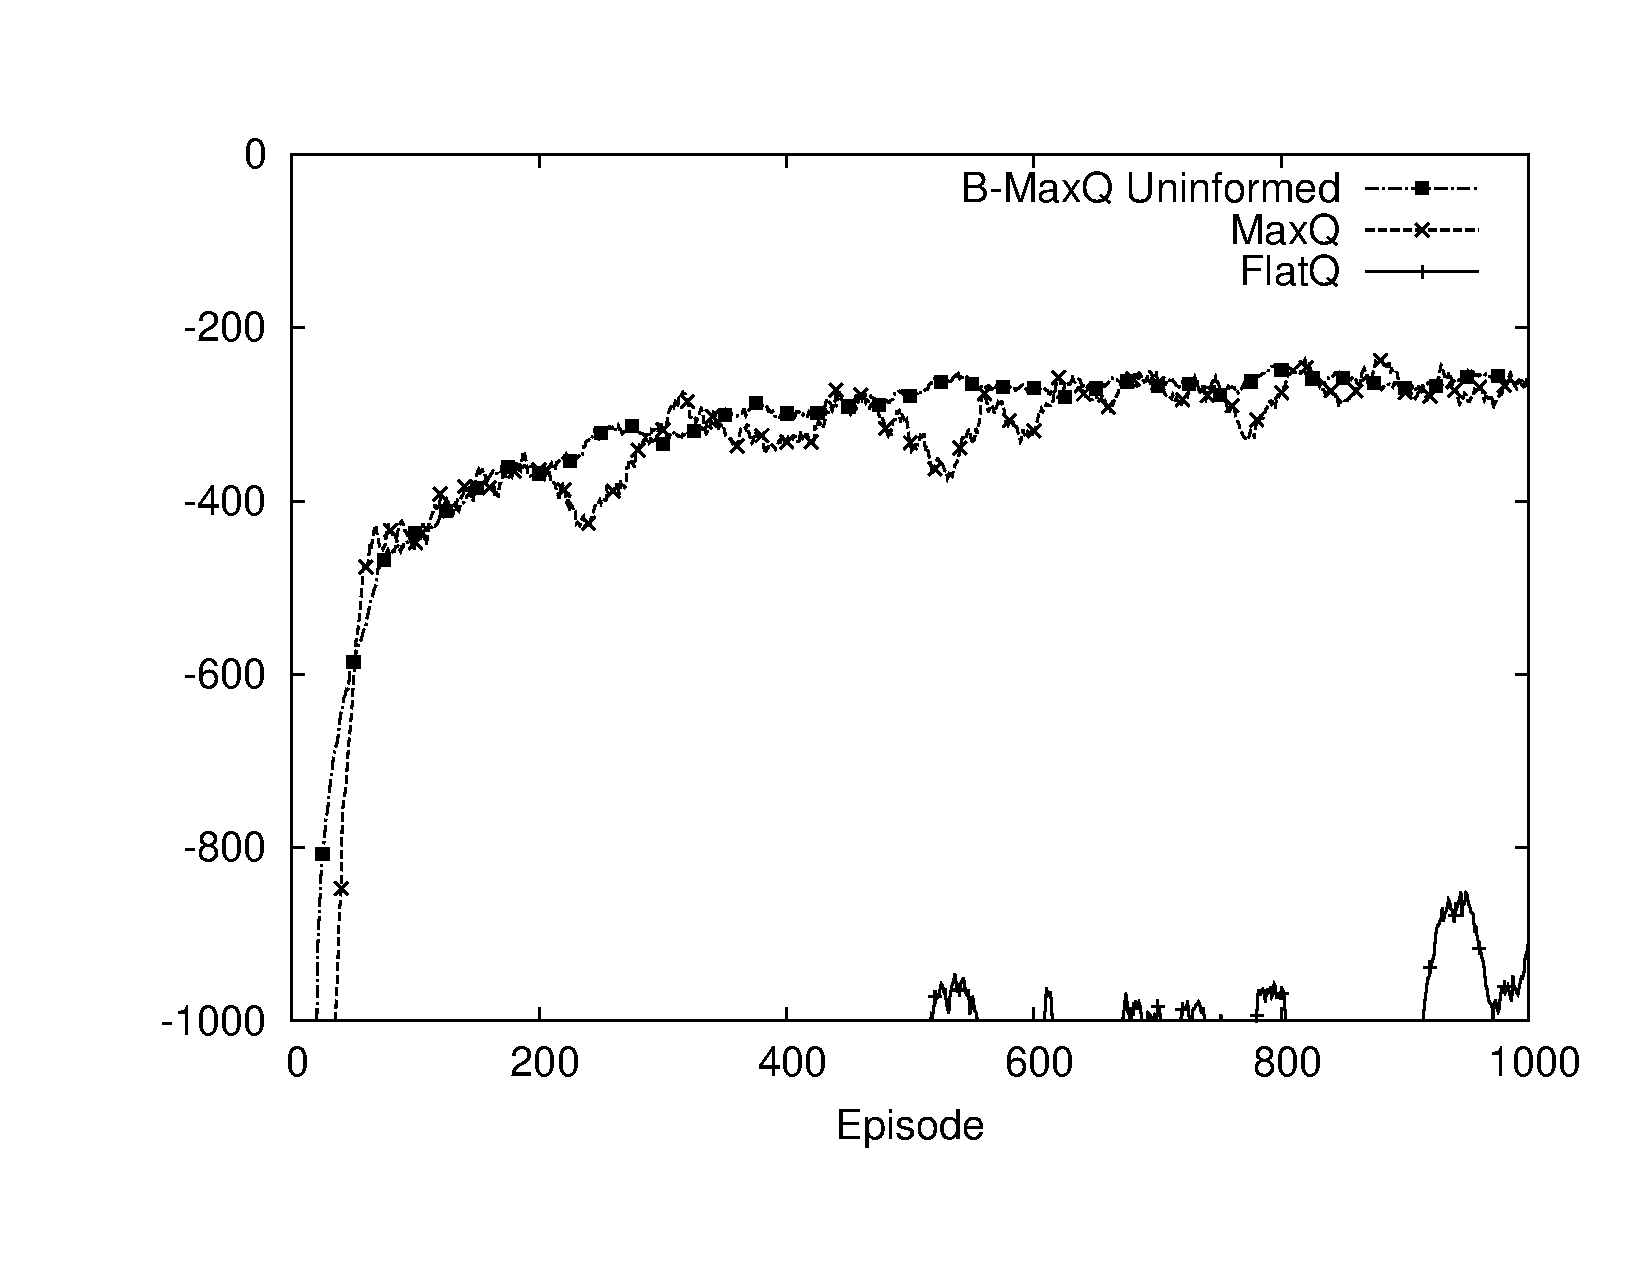
\includegraphics[trim=50 50 30 50, clip, scale=0.3]{exp/Wargus3322nb.pdf} \\
\end{tabular}

%\vspace{-0.3in}
\caption{Performance of different algorithms on {\sf Taxi-World} (top row) and {\sf Resource-collection} (bottom row). The
prefix ``B-'' denotes Bayesian, ``Uninformed/Good'' denotes the
prior and ``MB'' denotes model-based.}\label{fig:nopr}
\vspace{-0.2in}
\end{figure*}

\section{Empirical Evaluation}
\label{sec:expts}

In this section, we evaluate our approach and test four hypotheses:
First, does incorporating model-based priors help speed up the
convergence of {\sc maxq} to the optimal policy? Second, how does the
task hierarchy interact with the prior? Does the task hierarchy still
matter if very good priors are available for primitive actions? Third,
how does Bayesian {\sc maxq} compare to standard (flat) Bayesian RL? Does
Bayesian RL perform better (in terms of computational time) if a task
hierarchy is available? Finally, can our approach effectively learn
pseudo-rewards and policies that are hierarchically optimal?
% \begin{figure}
% \begin{tabular}{cc}
% \hspace{-0.5in}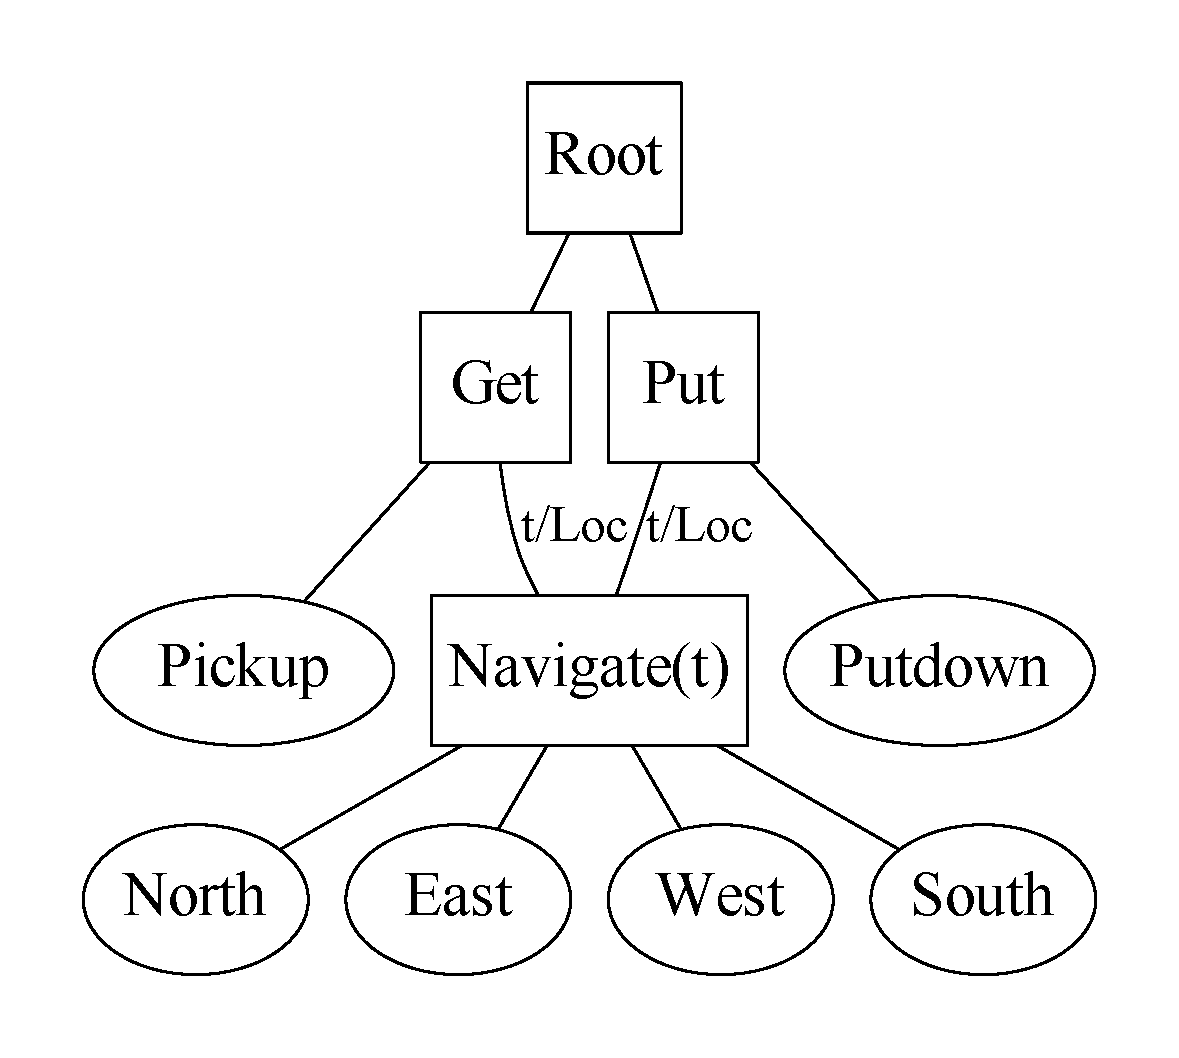
\includegraphics[scale=0.4]{task/Taxi-Hierarchy.pdf}&
% \hspace{-0.5in}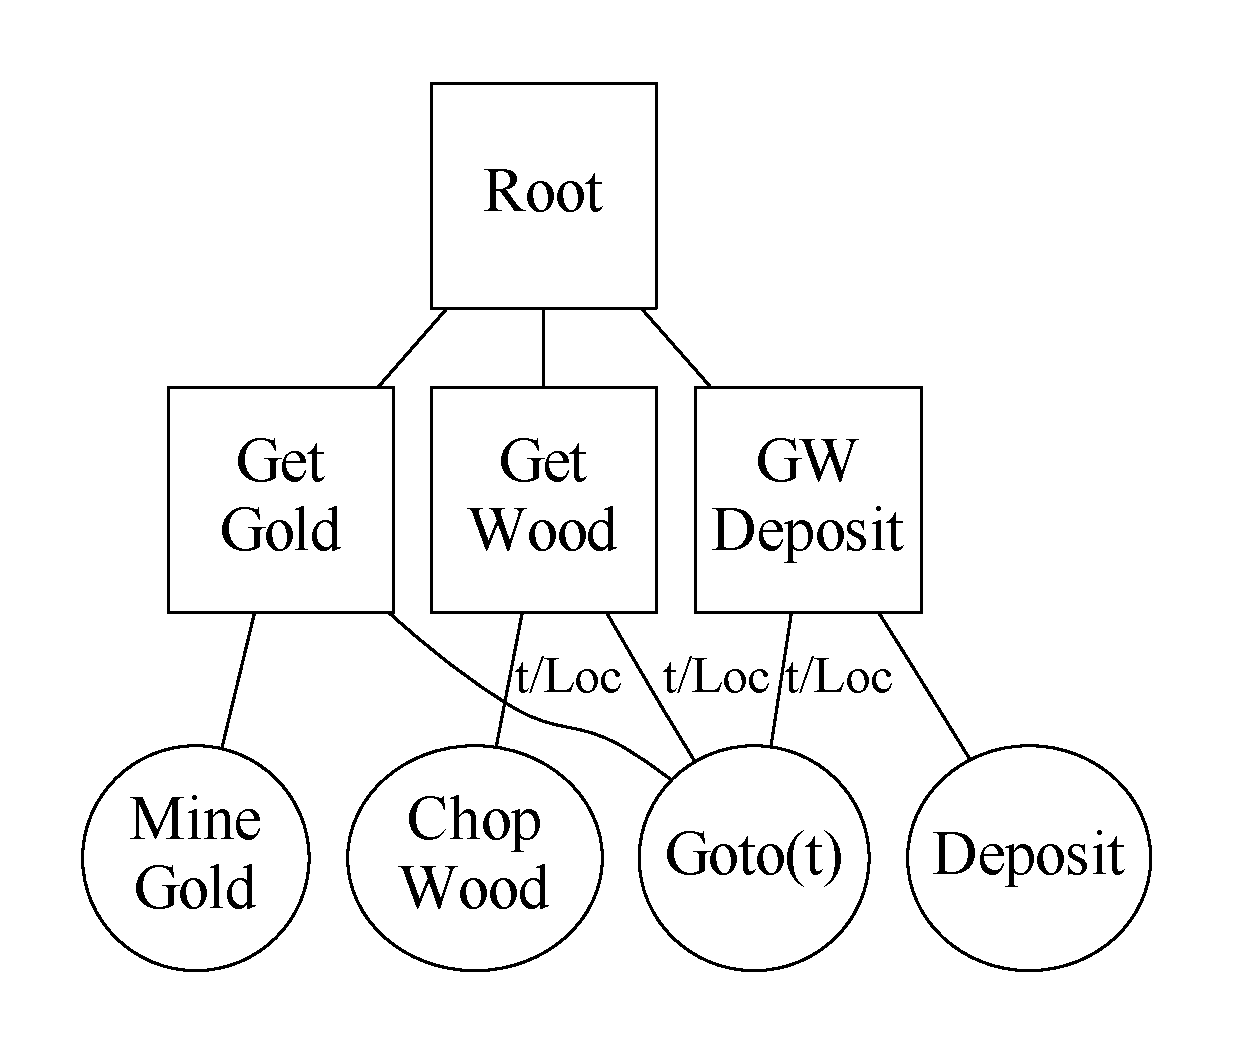
\includegraphics[scale=0.4]{task/Wargus-Hierarchy.pdf}\\
% \end{tabular}
% \caption{Task Hierarchies for {\sf Taxi-world} and {\sf Resource-collection}.}\label{fig:tasks}
% \vspace{-0.2in}
% \end{figure}

We first focus on evaluating the first three hypotheses using domains
where a zero pseudo-reward results in hierarchical optimality. To
evaluate these hypotheses, we use two domains: the 
fickle version of {\sf Taxi-World}~\cite{d-hrl-00} (625 states) and {\sf
  Resource-collection}~\cite{mehta.icml08} (8265 states). In {\sf Taxi-World}, the
agent controls a taxi in a grid-world that has to pick up a passenger
from a source location and drop them off at their destination. The
state variables consist of the location of the taxi and the source and
destination of the passenger. The actions available to the agent
consist of navigation actions and actions to pickup and putdown the
passenger.  The agent gets a reward of +20 upon completing the task, a
constant -1 reward for every action and a -10 penalty for an erroneous
action. Further, each navigation action has a 15\% chance of moving in
a direction orthogonal to the intended move. The {\sf
  Resource-collection} domain is inspired by real-time strategy games
where one component involves collecting resources from a map. We
simulate this through a grid world environment where the agent
controls a unit that can harvest gold and chop wood. Here the state
variables consist of the location of the agent, what the agent is
carrying, whether a goldmine or forest is adjacent to its current
location and whether a desired gold or wood quota has been met. The
actions available to the agent are to move to a specific location,
chop gold or harvest wood, and to deposit the item it is carrying (if
any). 
% To make the task tractable we limit the set of possible moves to
% a set of four locations adjacent to each goldmine, forest or deposit
% location. 
As before, for each navigation action the agent has a
probability of moving to a random location with 0.3 probability. 
% Further, in this
% domain, there may be multiple goldmines and multiple forests and
% multiple locations next to each goldmine and forest, so the action
% space is large. 
In our experiments, the map contains two
goldmines and two forests, each containing two units of gold and two
units of wood, and the gold and wood quota is set to three each. The
agent gets a +50 reward when it meets the gold/wood quota, a constant
-1 reward for every action and an additional -1 for erroneous actions
(such as trying to deposit when it is not carrying anything).
% The task hierarchies  are shown in
% Figure~\ref{fig:tasks}.

% \begin{figure*}[ht]
% \begin{tabular}{cc}
% %\hspace{-1in}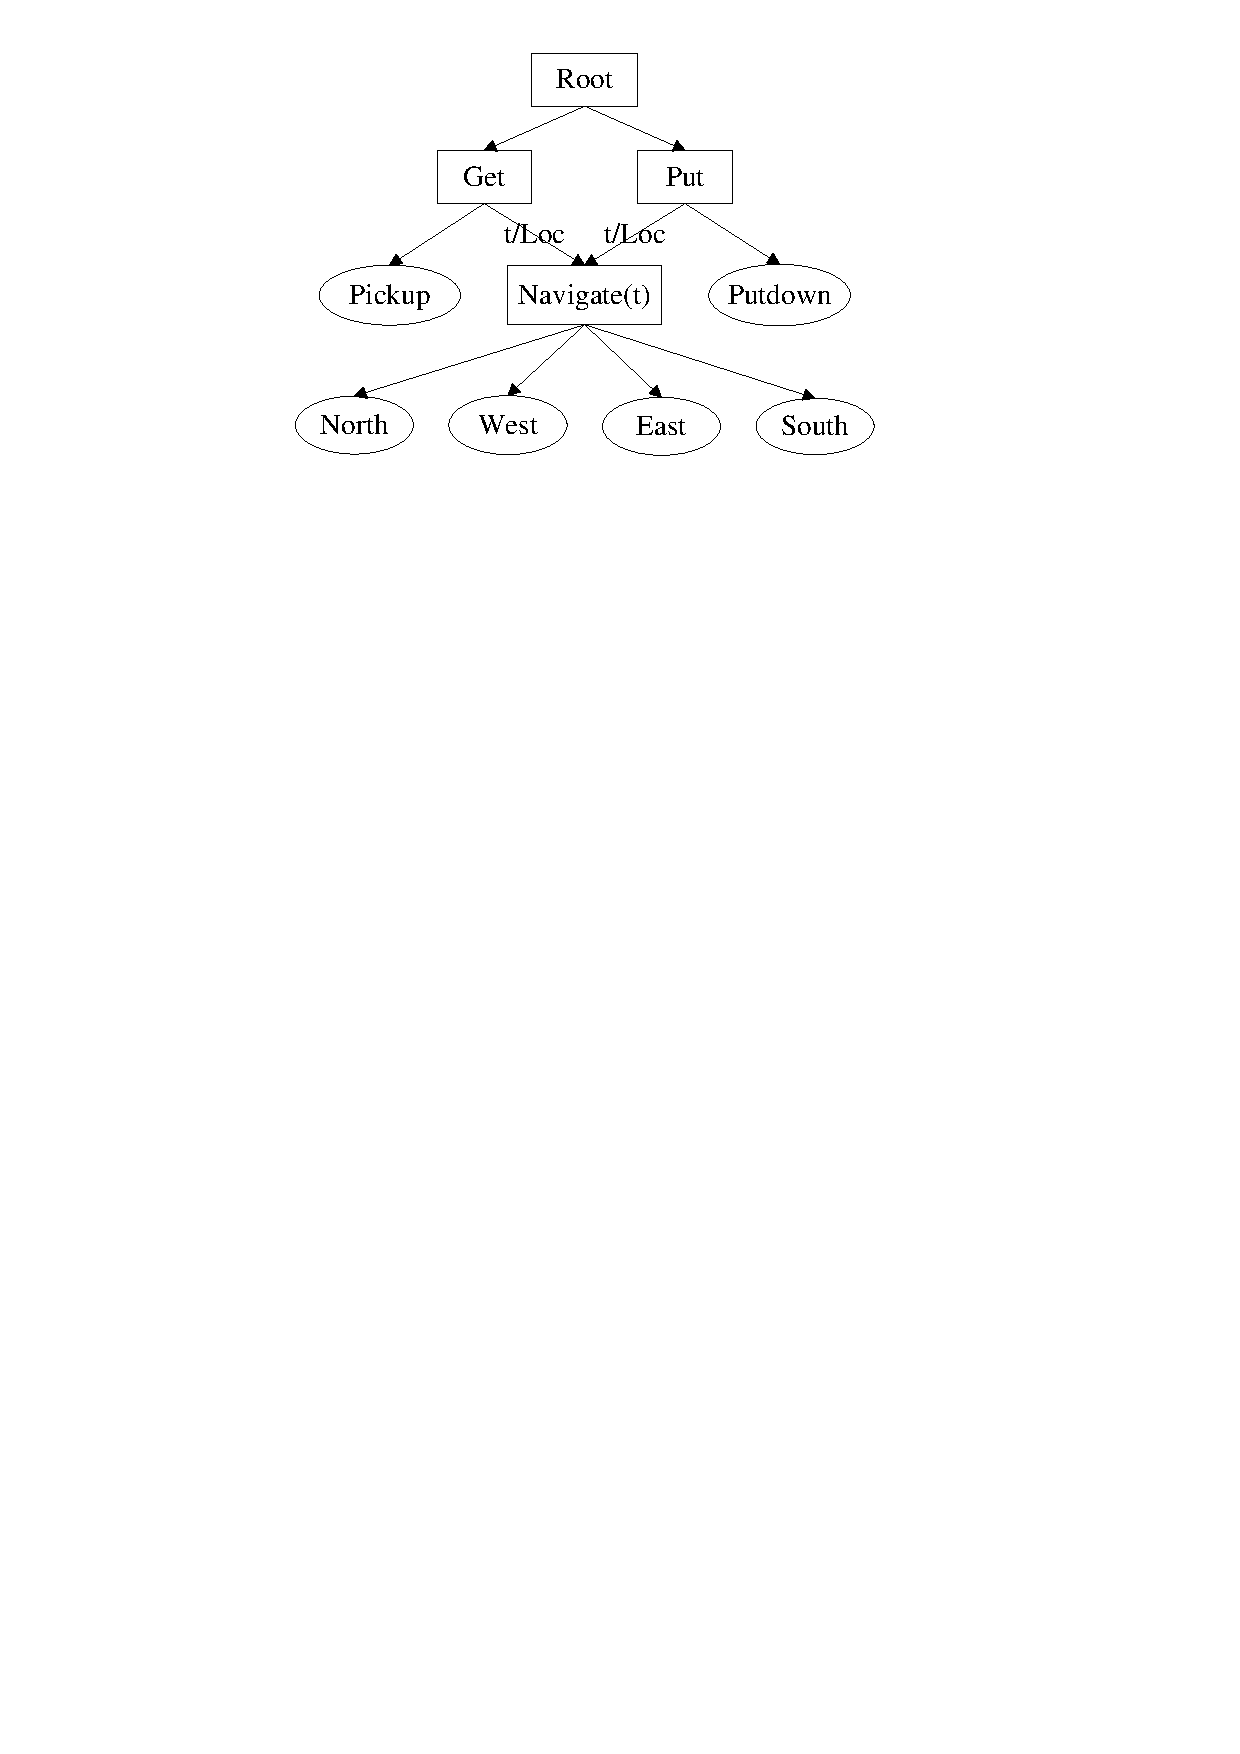
\includegraphics[scale=0.6]{Taxi-Hierarchy.pdf} &
% %\hspace{-2.5in}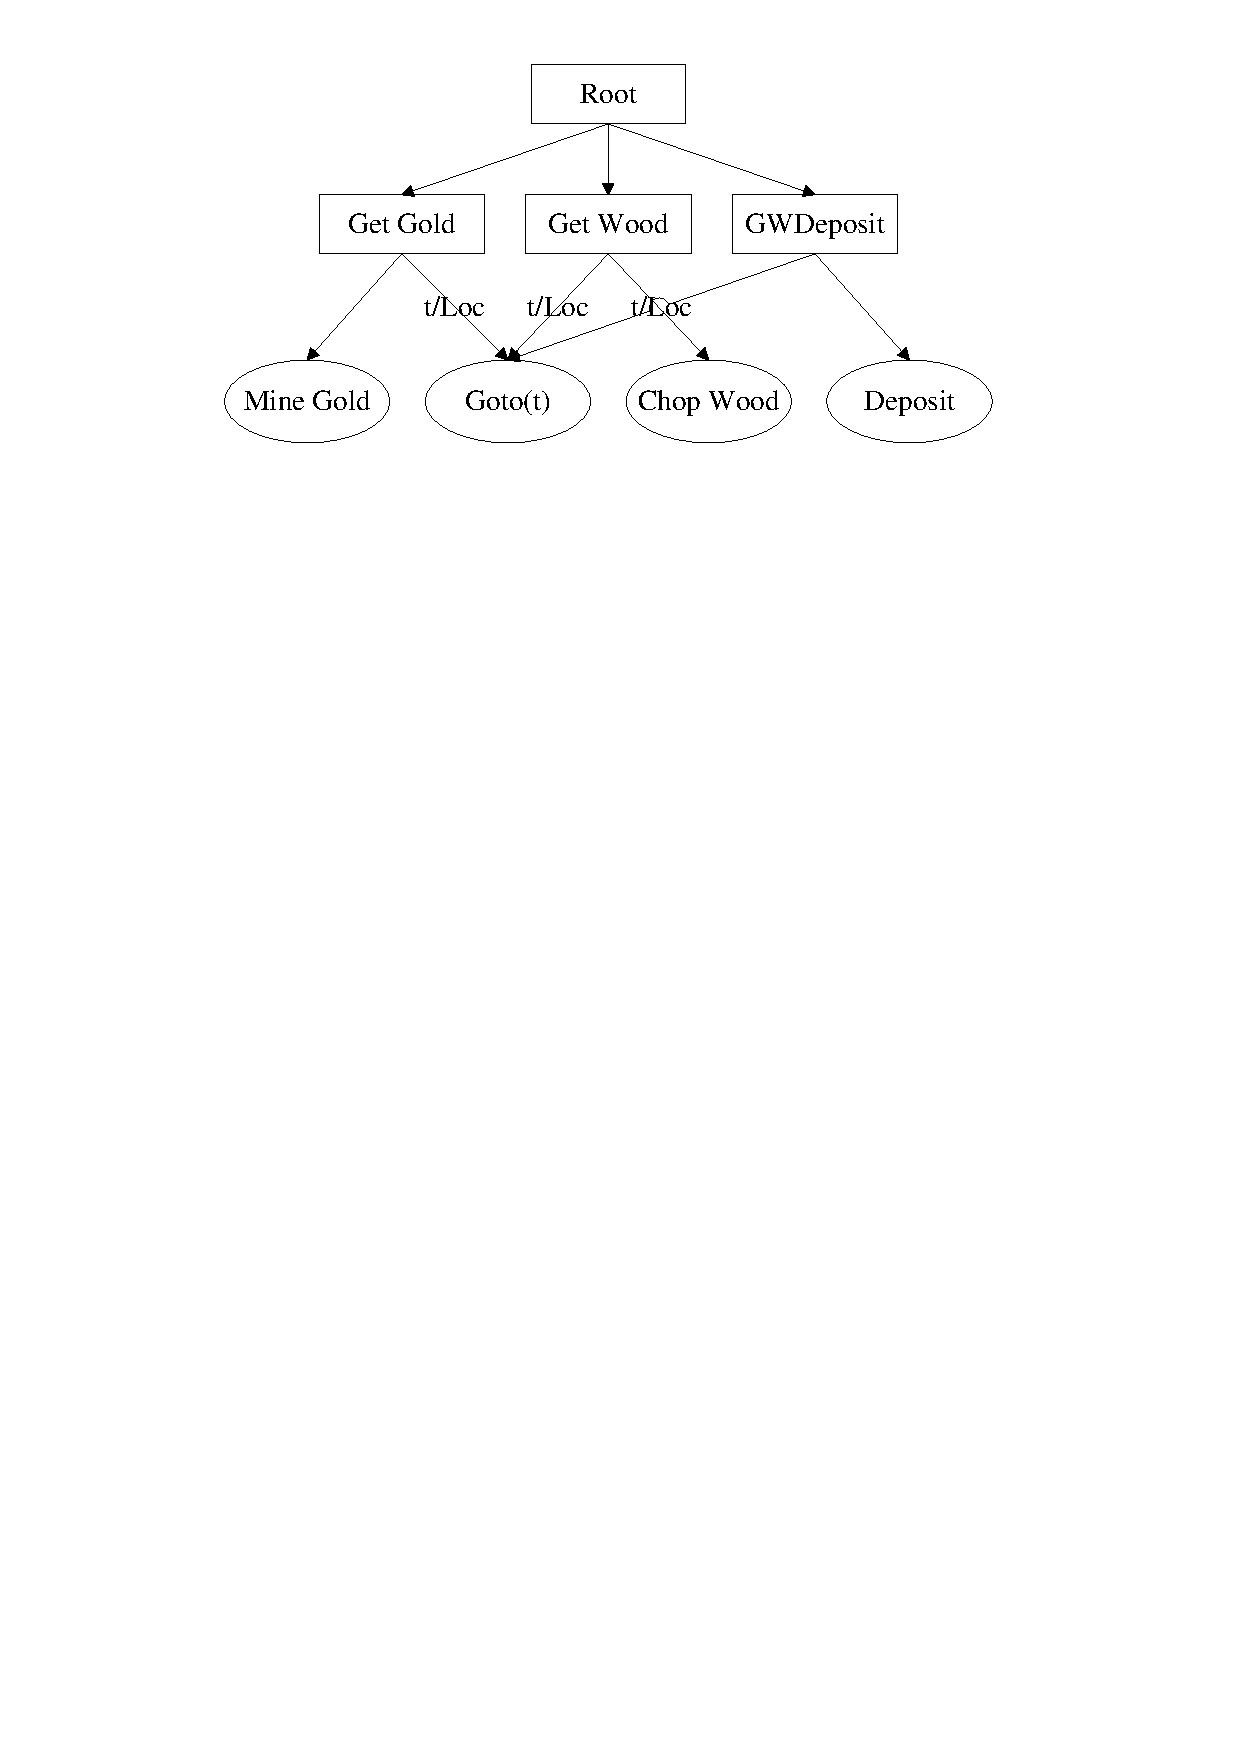
\includegraphics[scale=0.6]{Wargus-Hierarchy.pdf}\\
% %\vspace{-5.2in}
% & \multirow{2}{*}{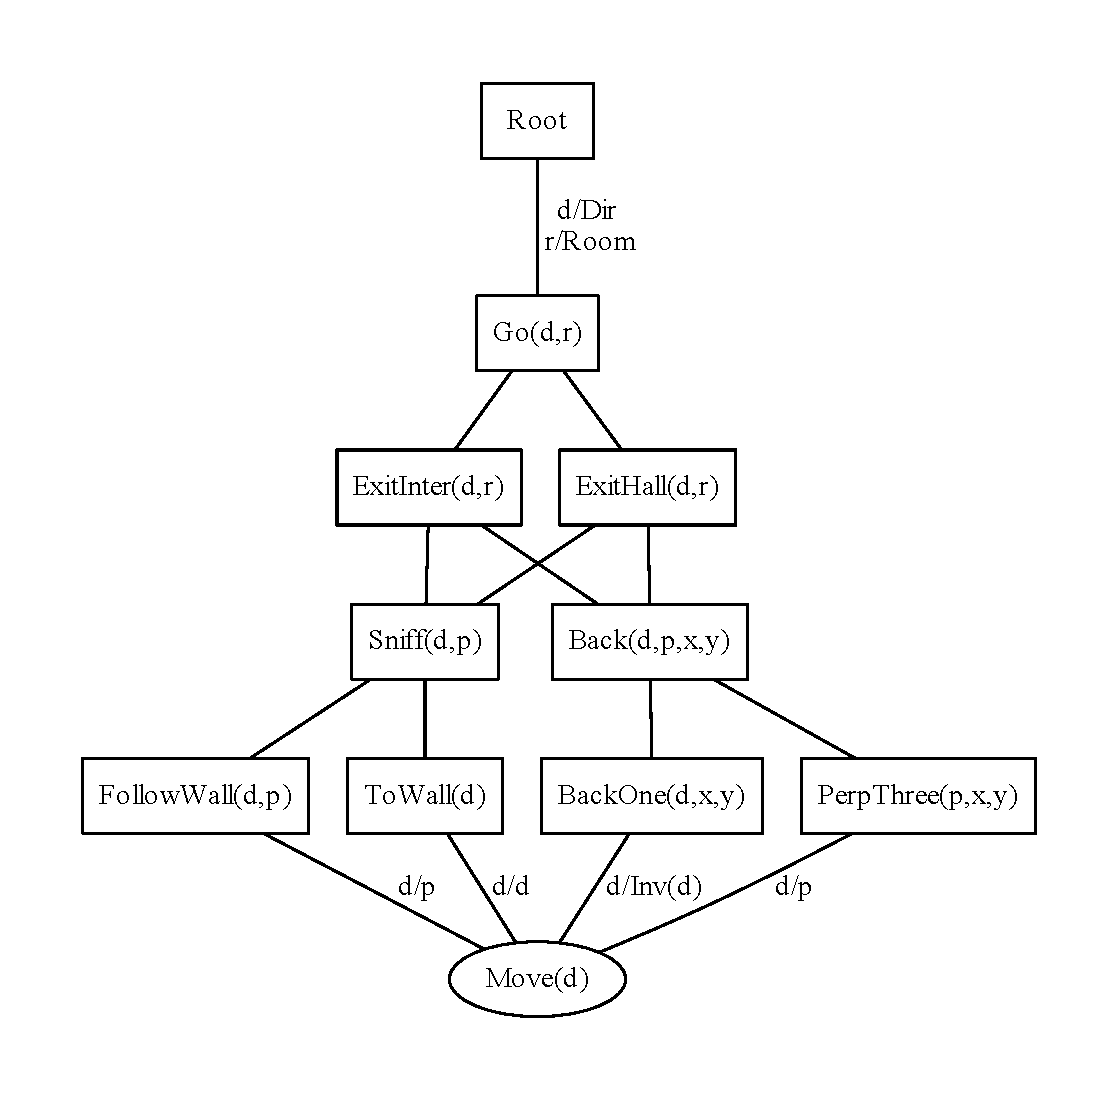
\includegraphics[scale=0.5]{task/Hallway-Hierarchy.pdf}} \\
% 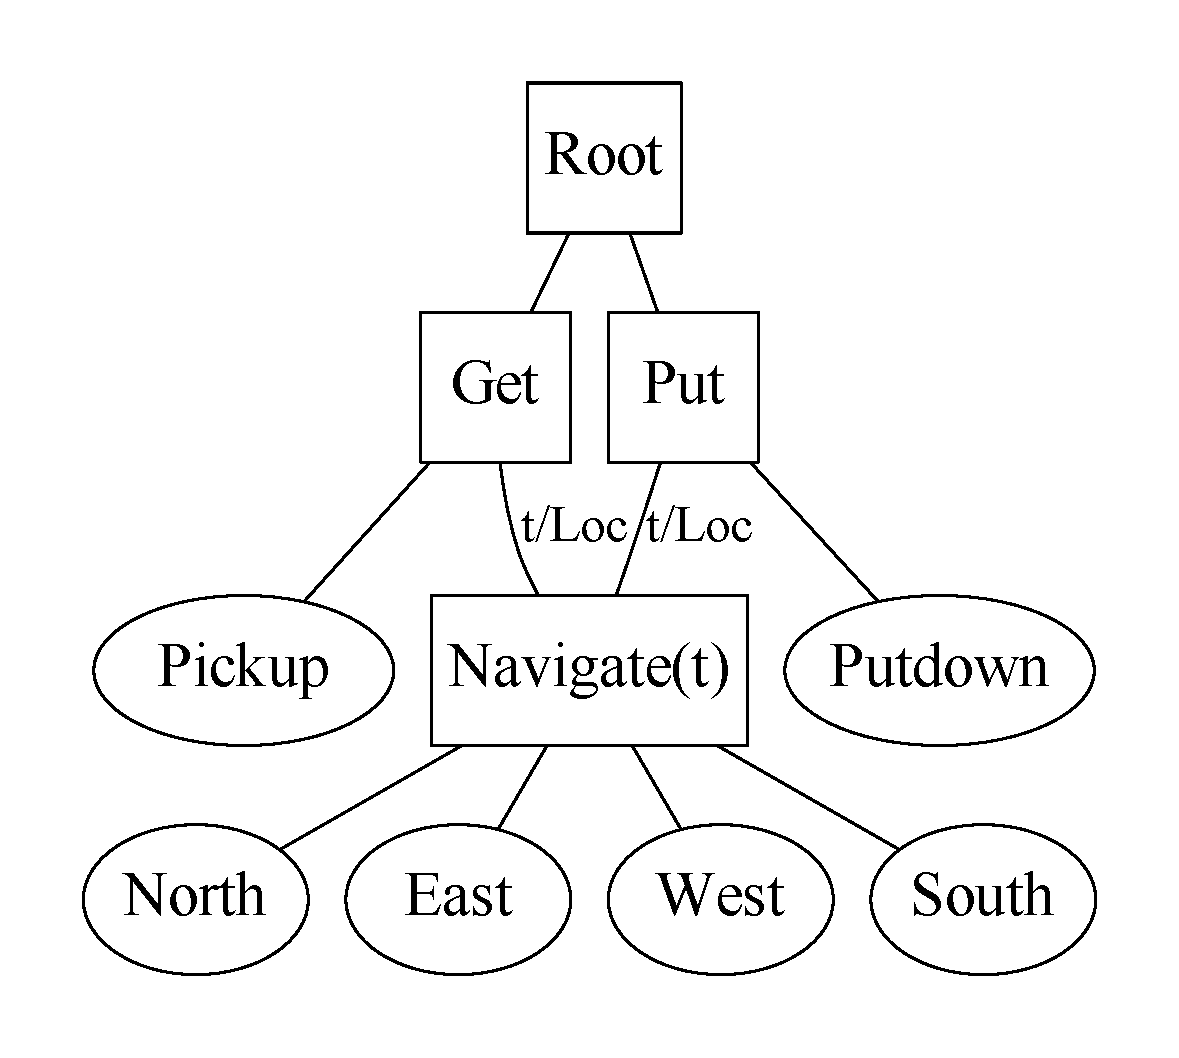
\includegraphics[scale=0.4]{task/Taxi-Hierarchy.pdf} & \\
% 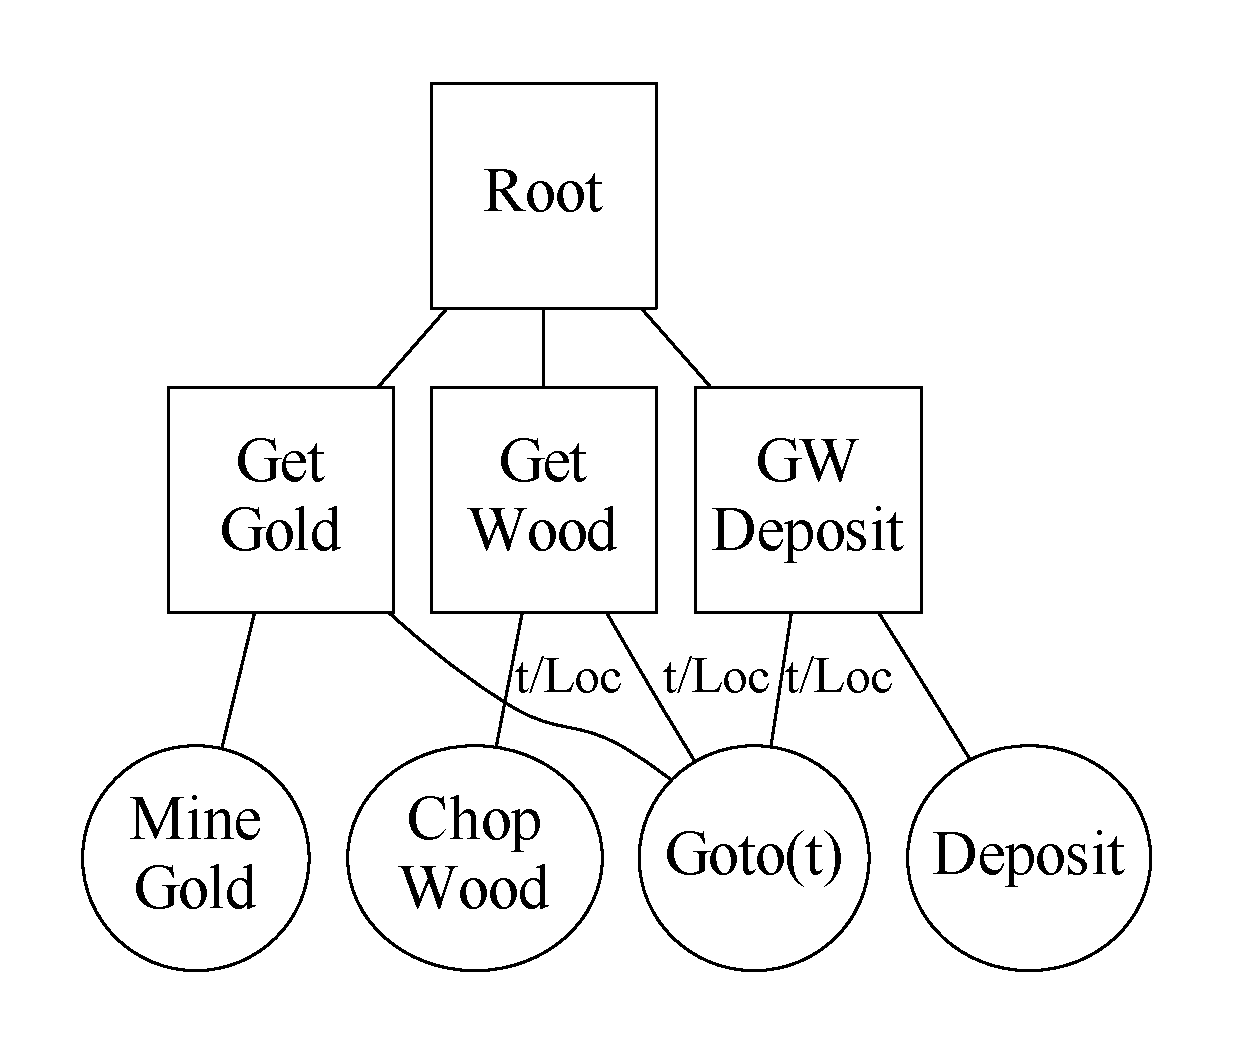
\includegraphics[scale=0.4]{task/Wargus-Hierarchy.pdf} & \\
% \end{tabular}
% \caption{Task Hierarchies for {\sf Taxi-world} (top-left), {\sf Resource-collection} (bottom-left) and {\sf Hallway} (right)\\
% Note that in subtasks Sniff and Back of Hallway, parameter $p$ is perpendicular to $r$, $(x, y)$ is the location of agent when Back is called.}\label{fig:tasks}
% \end{figure*}



For the Bayesian methods, we use Dirichlet priors for
the transition function parameters and Normal-Gamma priors for the
reward function parameters. We use two priors: an uninformed prior,
set to approximate a uniform distribution, and a ``good'' prior where
a previously computed model posterior is used as the ``prior.''
% priors. The first case is an uninformed prior. Here the priors
%  are set to approximate a uniform distribution over model
% parameters. The second case is a ``good'' prior. In this case, we
% first run the Bayesian MAXQ approach for 1000 episodes on each
% problem, and use the estimated model posterior as the prior.
 The prior
distributions we choose are conjugate to the likelihood, so we can compute the
posterior distributions over the relevant parameters in closed form.
In general, this is not necessary; more complex priors could be used
as long as we can sample from the posterior distribution.
\renewcommand{\arraystretch}{1}
\begin{table}[t] \footnotesize

\caption{CPU time for methods on {\sf Taxi-World}.}

\label{tab:time}

\begin{center}

\begin{tabular}{| p{4cm} | l |}

\hline

\multirow{3}{*}{Method} & Time for \\

&500 Episodes (s)\\ \hline

Bayesian MaxQ, Uninformed Prior &179\\ 

Bayesian Model-based Q, Uninformed Prior &232\\ 

Bayesian MaxQ, Good Prior &14\\ 

Bayesian Model-based Q, Good Prior &119\\ 

Bayesian Model-based Q, Good Prior \& Comparable Simulations
&934 \\ 

MaxQ &1.15 \\

FlatQ &0.53 \\
\hline
\end{tabular}

\end{center}
\vspace{-0.2in}
\end{table}

The methods we use in this experiment are: (i) Flat Q, the standard,
non-Bayesian Q-learning algorithm, (ii) {\sc maxq-0}, the standard,
non-Bayesian Q-learning algorithm for {\sc maxq} with no pseudo-reward,
(iii) Bayesian model-based Q-learning with an uninformed prior and (iv) a ``good'' prior, (v) Bayesian {\sc maxq} (our proposed approach) with
an uninformed prior and (vi) with a ``good'' prior. In our implementation,
the Bayesian model-based Q-learning uses the same code as the Bayesian
{\sc maxq} algorithm, with a ``trivial'' hierarchy consisting of the Root
task with only the primitive actions as children. For the Bayesian methods, the update frequency $k$
was set to 50 for {\sf Taxi-World} and 25 for {\sf
  Resource-collection}. $Sim$ was set to 200 for Bayesian {\sc maxq} for
{\sf Taxi-World} and 1000 for Bayesian model-based Q, and to 1000 for
both for {\sf Resource collection}.
% We make two changes
% to the Bayesian MAXQ algorithm for efficiency: first, we use ``all
% states updating''~\cite{d-hrl-00}, where the completion function is
% updated fro all states seen in the child task rather than just the
% exit. Second, in Line~\ref{line:sample} in {\sc Recompute\_value}, we
% sample a model from the posterior~\cite{Strens}. We observed that, as
% noted by others~\cite{icml2007}, the convergence behavior can be
% improved by sampling an approximately MAP model. We approximate this
% by computing the MAP model from our posterior, and then using an
% $\epsilon$-greedy hierarchical policy to select actions. 
The results
 are shown in Figure~\ref{fig:nopr}. 

From these results, comparing the Bayesian versions of {\sc maxq} to 
standard {\sc maxq}, we observe that for {\sf Taxi-World}, the
Bayesian version converges faster to the optimal policy even with the
uninformed prior, while for {\sf Resource-collection}, the convergence
rates are similar. When a good prior is available, convergence is
very fast (almost immediate) in both domains. Thus, the availability
of model priors can help speed up convergence in many cases for HRL.

Next, we compare the Bayesian {\sc maxq} approach to ``flat'' Bayesian
model-based Q learning. We note that in {\sf Taxi-World}, with uninformed
priors, though the ``flat'' method initially does worse, it soon
catches up to standard {\sc maxq} and then to Bayesian {\sc maxq}. This is
probably because in this domain, the primitive models are relatively
easy to acquire, and the task hierarchy provides no additional
leverage. For {\sf Resource-collection}, however, 
% Note that for the ``good'' prior in this task, Bayesian MAXQ
% and flat Bayesian model-based learning do about equally well. This
% indicates that in some cases the availability of a good model prior
% may reduce the need for a task hierarchy. However, this does not
% always happen, as shown in the {\sf Resource-collection} domain, where
even with a good prior, ``flat'' Bayesian model-based Q does not
converge. The difference is that in this case, the task hierarchy
encodes extra information that cannot be deduced just from the models.
In particular, the task hierarchy tells the agent that good policies
consist of gold/wood collection moves followed by deposit moves. Since
the reward structure in this domain is very sparse, it is difficult to
deduce this even if very good models are available. Taken together,
these results show that task hierarchies and model priors can be
complementary: in general, Bayesian {\sc maxq} outperforms both flat
Bayesian RL and {\sc maxq} (in speed of convergence, since here {\sc maxq} can
learn the optimal policy).

% Thus, good priors may not be sufficient to
% guarantee fast convergence---task hierarchies can encode additional
% information about good policies that help convergence even in the presence
% of good priors. However, if no such policy information is encoded by
% the hierarchy (e.g. the hierarchy allows all ``legal'' policies),
% then a good prior on the model reduces or eliminates the convergence advantage of
% HRL over flat RL.
\begin{figure}
\centerline{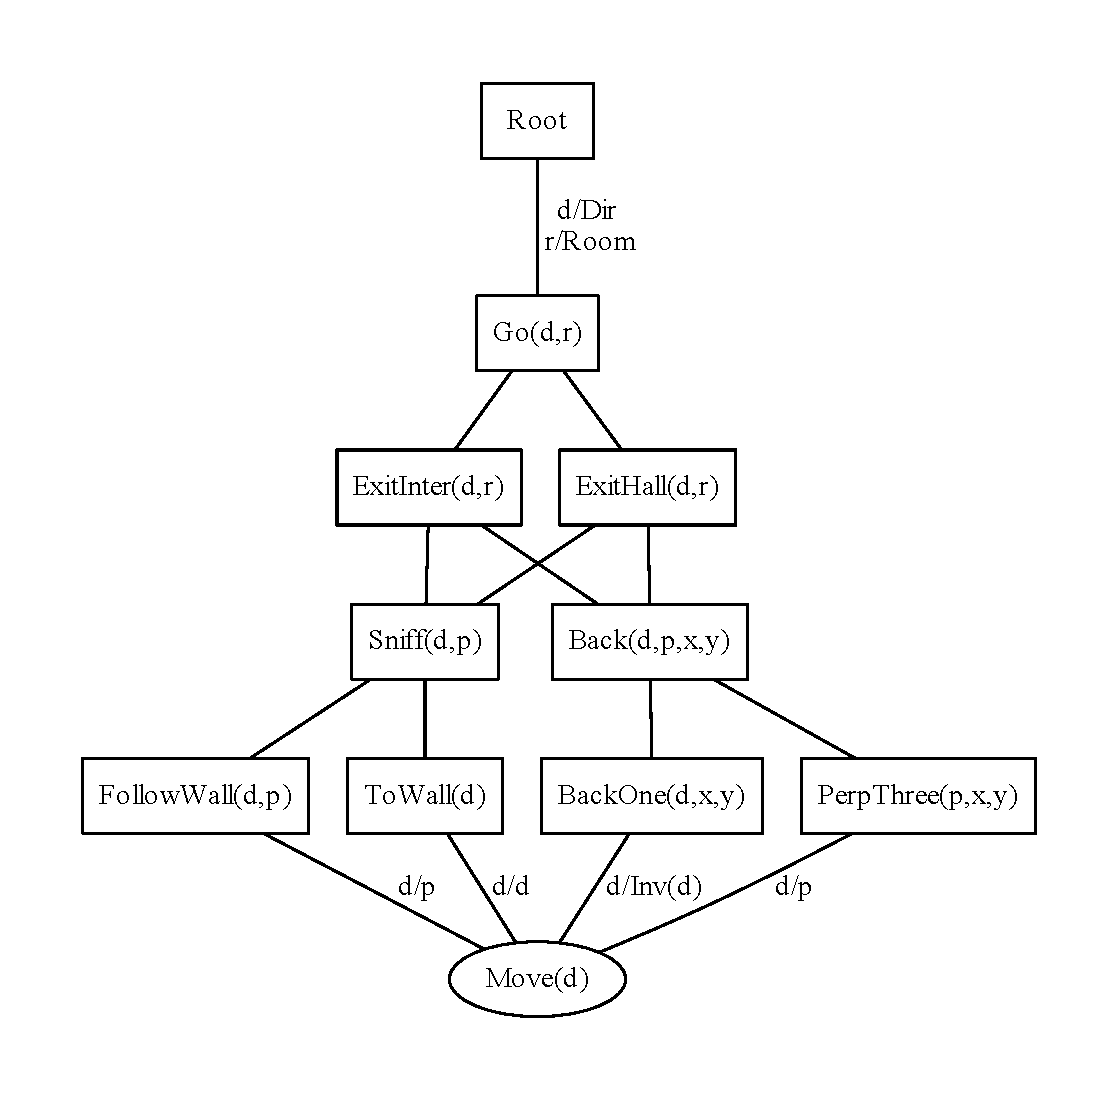
\includegraphics[scale=0.5]{task/Hallway-Hierarchy.pdf}}
\vspace{-0.3in}\caption{Task Hierarchy for {\sf Hallway}.}\label{fig:hallway}
\vspace{-0.2in}\end{figure}

\renewcommand{\arraystretch}{0}
\begin{figure*}[ht]
\centering
\begin{tabular}{cc}
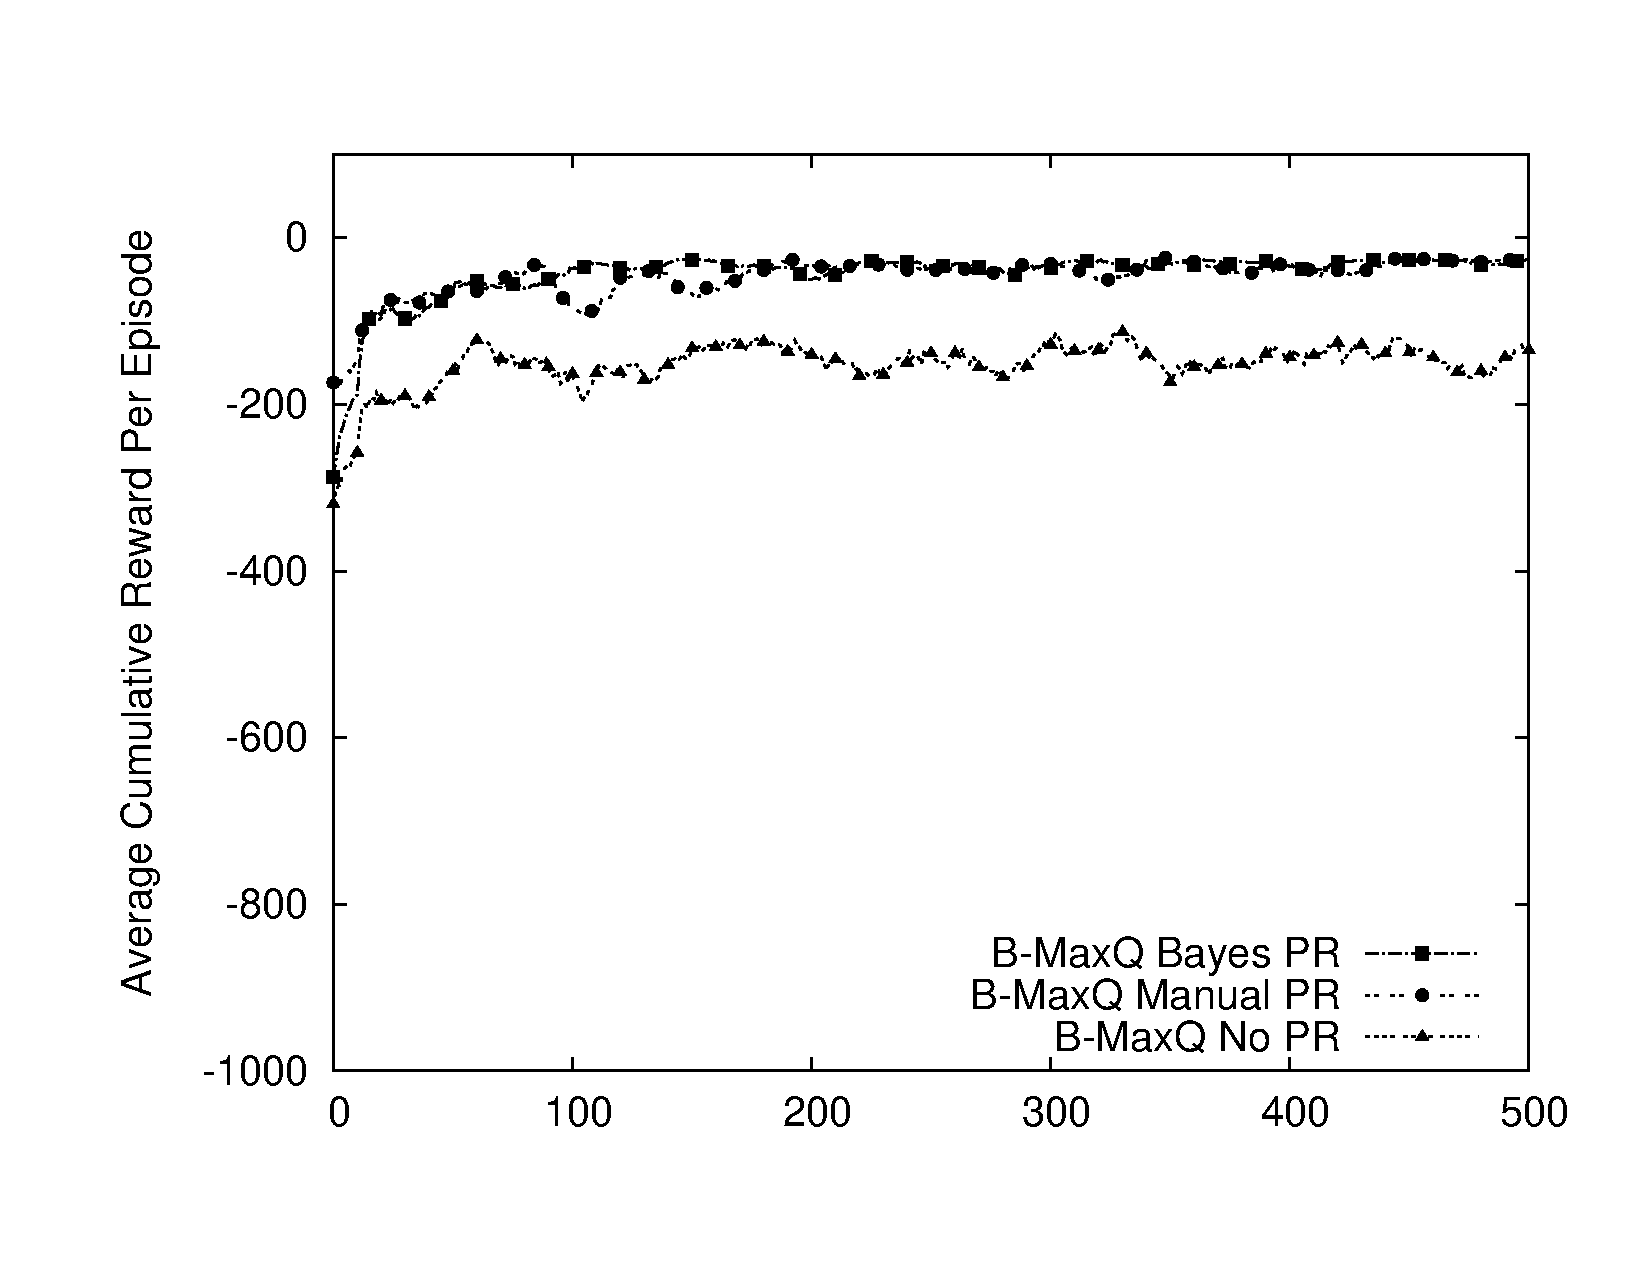
\includegraphics[trim=50 50 30 50, clip, scale=0.3]{exp/Taxi_Modified_b.pdf} & 
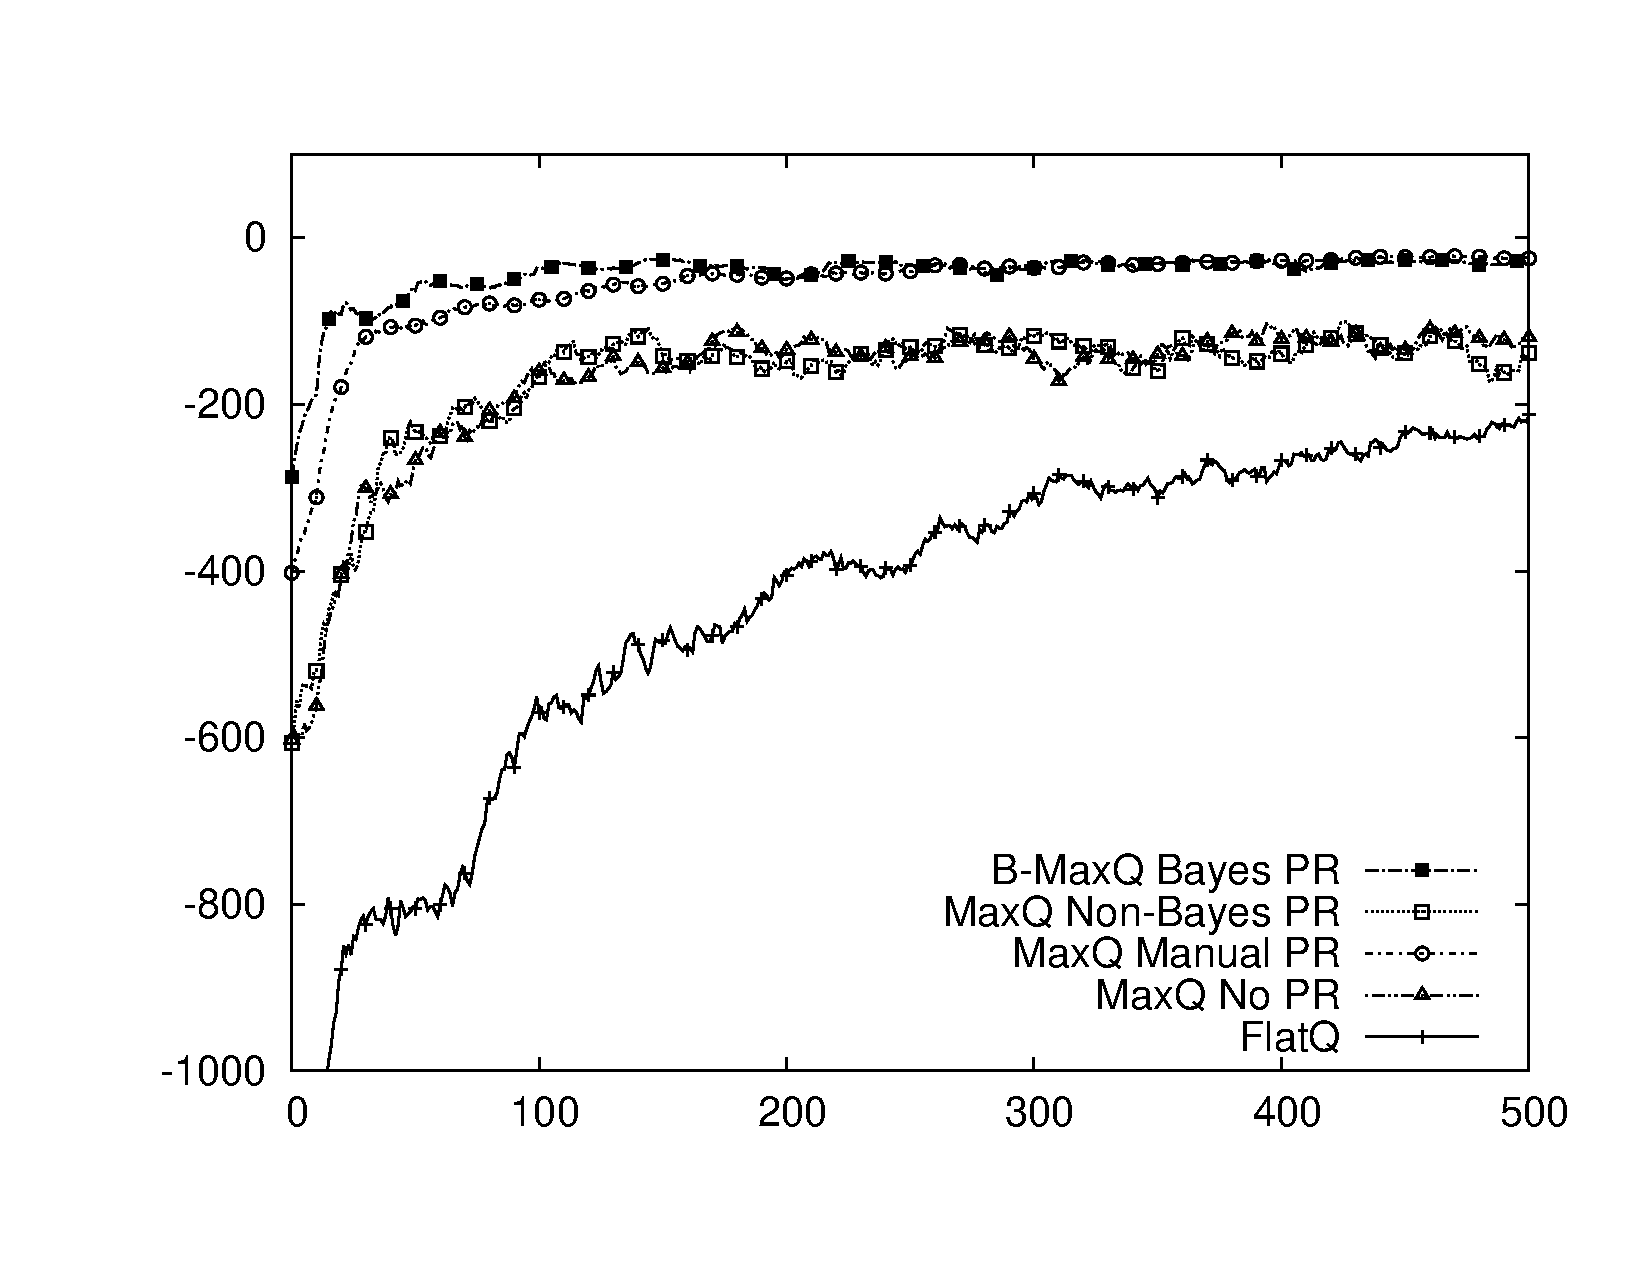
\includegraphics[trim=50 50 30 50, clip, scale=0.3]{exp/Taxi_Modified_nb.pdf} \\
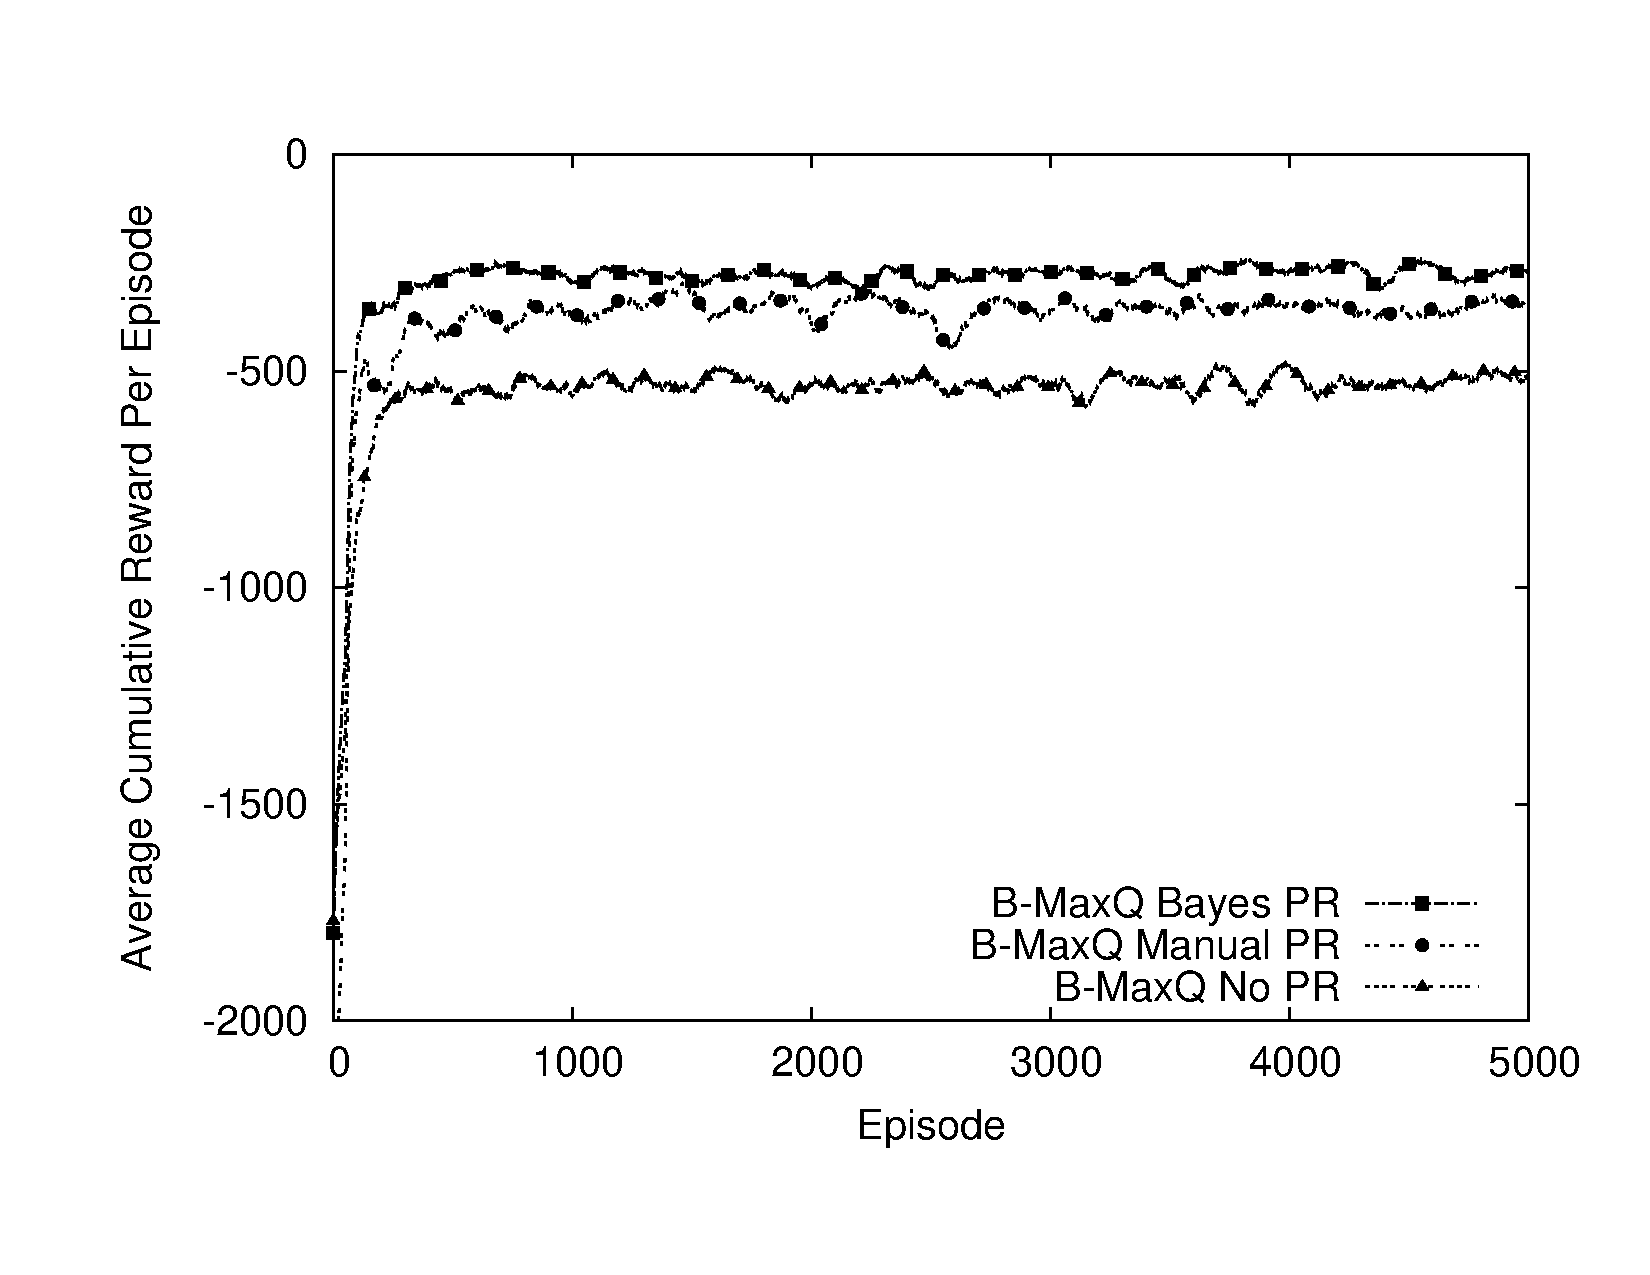
\includegraphics[trim=50 50 30 50, clip, scale=0.3]{exp/Hallwayb.pdf} & 
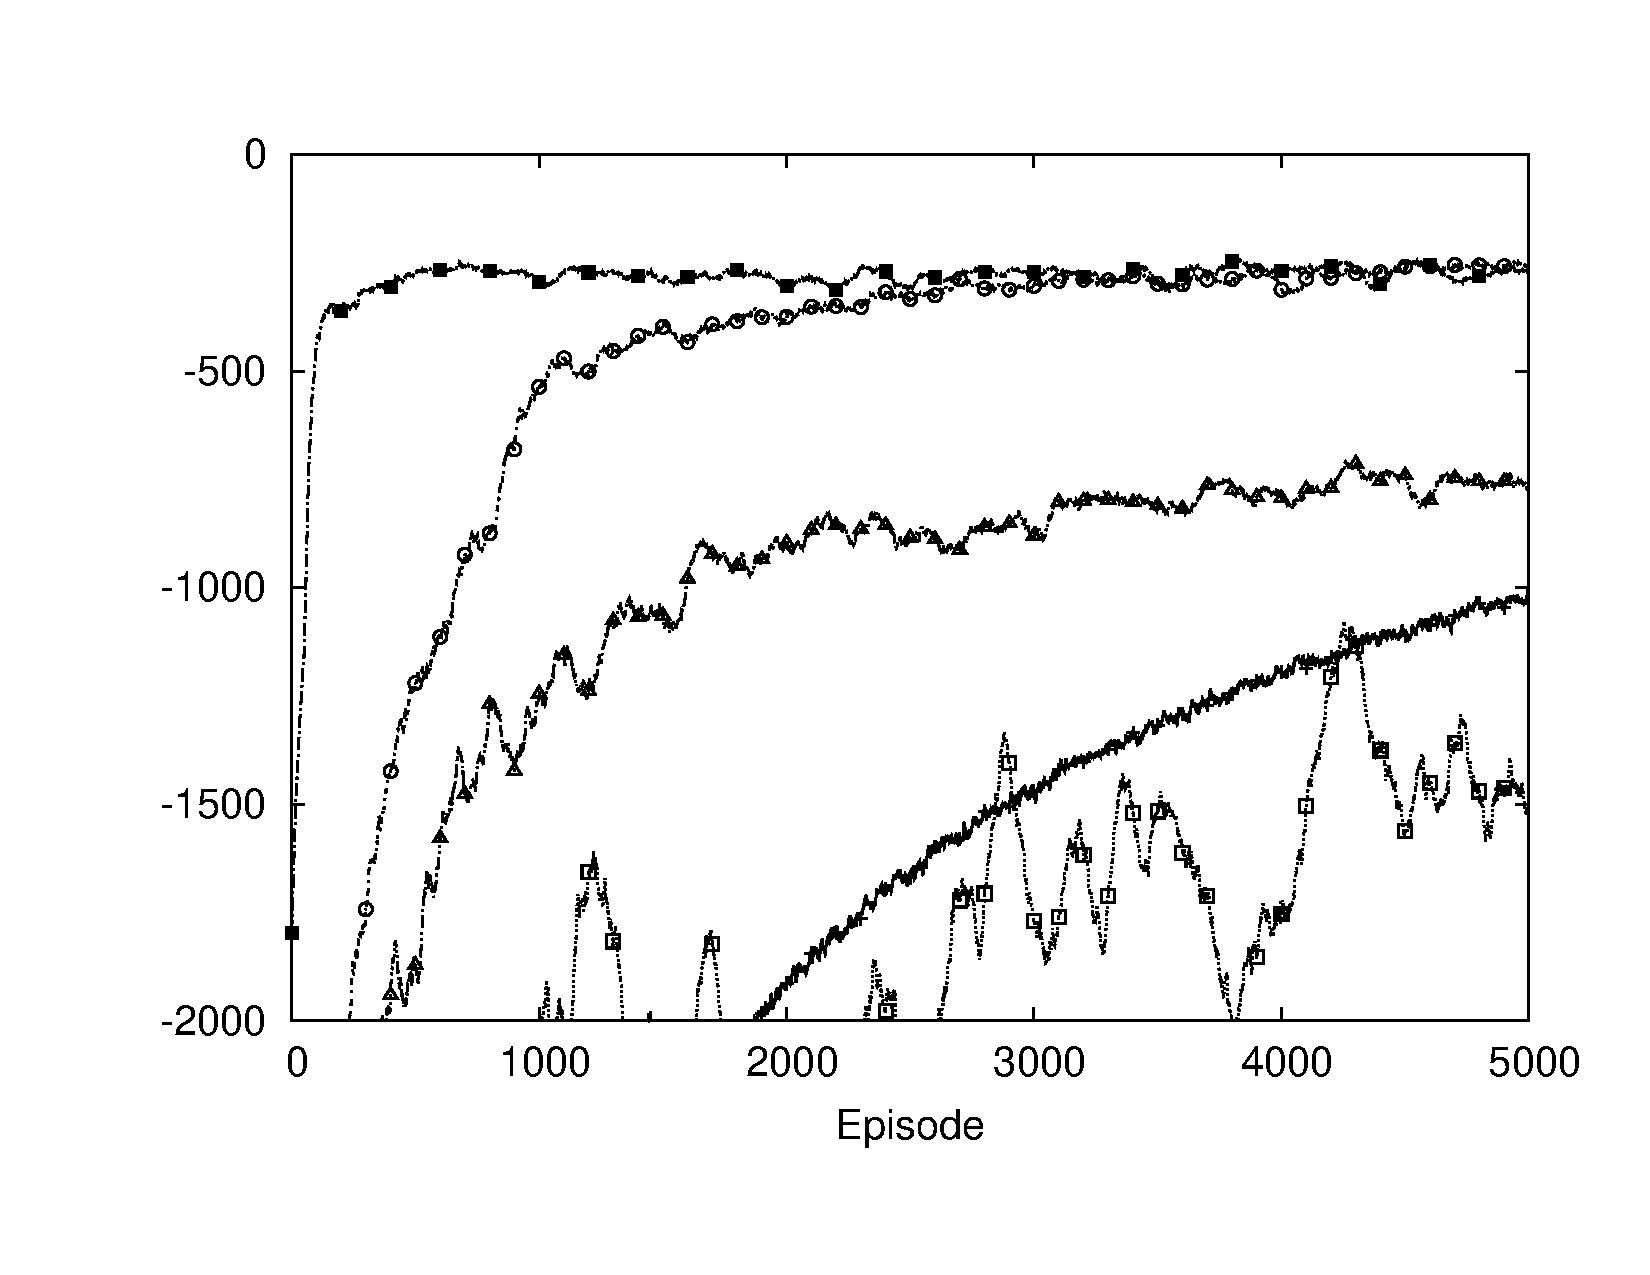
\includegraphics[trim=50 50 30 50, clip, scale=0.3]{exp/Hallwaynb.pdf} \\
\end{tabular}
%\vspace{-0.3in}
\caption{Performance of different algorithms on {\sf Modified-Taxi-World} (top row) and {\sf Hallway} (bottom row). The
prefix ``B-'' denotes Bayesian, ``PR'' denotes Pseudo Reward.}\label{fig:pr}
\vspace{-0.2in}\end{figure*}

Next, we compare the time taken by the different approaches in our
experiments in {\sf Taxi-World} (Table~\ref{tab:time}). As expected, the
Bayesian RL approaches are significantly slower than the non-Bayesian
approaches. However, out of the Bayesian methods, the Bayesian {\sc maxq} approaches are
significantly faster than the flat Bayesian model-based
approaches. This can be attributed to the fact that for the flat case,
during the simulation in {\sc Recompute\_value}, a much larger task
needs to be solved, while the Bayesian {\sc maxq} approach is able to take
into account the structure of the hierarchy to only simulate subtasks
as needed, which ends up being much more efficient. However, we note
that we allowed the flat Bayesian model-based approach 1000 episodes
of simulation as opposed to 200 for Bayesian {\sc maxq}. Clearly this
increases the time taken for the flat cases. But at the same time,
this is necessary: the ``Comparable Simulations'' row (and curve in
Figure~\ref{fig:nopr} top left) shows that, if the simulations are reduced to
250 episodes for this approach, the resulting values are no longer reliable and the performance of
the Bayesian flat approach drops sharply. Thus, taking advantage of
the hierarchical task decomposition helps reduce the computational cost of
Bayesian RL.


% \begin{table*}[t]
% \caption{CPU time taken by various methods on {\sf Taxi-world}.}
% \label{tab:time}
% \begin{center}
% \begin{tabular}{| p{4cm} | l | l | l | l | l |}
% \hline
% \multirow{5}{*}{Method} 	&Tot. Time  for	&\multicolumn{2}{|c|}{}  &\multicolumn{2}{|c|}{}			\\ 
% 						&500 Episodes 	&\multicolumn{2}{|c|}{Episodes with} 	 &\multicolumn{2}{|c|}{Episodes with}			\\
% 						&(s)				&\multicolumn{2}{|c|}{5-20 Steps}	&\multicolumn{2}{|c|}{70-120 Steps} 		\\ 
% 						&				&\multicolumn{2}{|c|}{(near-optimal)}		&\multicolumn{2}{|c|}{(suboptimal)}				\\ \cline{3-6}
% 						&
%                                                 &Avg Time (ms)	&Count
%                                                 &Avg Time (ms)	&Count \\ \hline
						
% Bayesian MaxQ, Uninformed Prior	&179	&21		&81 		&332  	&39 				\\ \hline
% Bayesian Model-based Q, Uninformed Prior	&232	&162 	&211 	&851	&25 					\\ \hline
% Bayesian MaxQ, Good Prior		&14		&17 		&209 	&84 		&3 				\\ \hline
% Bayesian Model-based Q, Good Prior		&119	&172 	&316 	&- 		&0 				\\ \hline
% Bayesian Model-based Q, Good Prior \& Comparable Simulations 									&934	&- 		&0		&687	&56		\\ \hline
% MaxQ							&0.53	&- 		&0		&1.49 	&171				\\ \hline
% Flat Q							&1.15	&- 		&0		&0.37	&18			\\ \hline
% \end{tabular}
% \end{center}
% \end{table*}



Finally we evaluate how well our approach estimates pseudo-rewards. Here we use two domains: a {\sf Modified-Taxi-World} and a
{\sf Hallway} domain~\cite{d-hrl-00,parr:thesis} (4320 states). In {\sf Modified-Taxi-World}, We allow dropoffs at any one of the four specific locations and do not provide a reward for task
termination. Thus the Navigate subtask needs a pseudo-reward
(corresponding to the correct dropoff location) to learn a good policy.
The {\sf Hallway} domain consists of a maze with a large scale
structure of hallways and intersections. The agent has stochastic movement actions. The task hierarchy is shown in Figure~\ref{fig:hallway}. 

For these experiments, we use uninformed priors on the
environment model. The pseudo-reward priors are set to prefer each
exit from a subtask equally. The baselines we
use are: (i) Bayesian {\sc maxq} and {\sc maxq} with fixed zero pseudo-reward, (ii)
Bayesian {\sc maxq} and {\sc maxq} with fixed manually set pseudo-reward, (iii)
flat Q and (iv) {\sc maxq} with a non-Bayesian pseudo-reward update. This last
method tracks pseudo-reward just as our approach; however, instead of
a Bayesian update, it updates the pseudo-reward using a temporal
difference update, treating it as a simple value function. The results
 are shown in Figure~\ref{fig:pr}.

From these results, we first observe that the methods with zero
pseudo-reward always do worse than those with ``proper'' pseudo-reward,
indicating that in these cases the recursively optimal policy is not
the hierarchically optimal policy. When a pseudo-reward is manually
set, in both domain, {\sc maxq} converges to better policies. We observe that
in each case, the Bayesian {\sc maxq} approach is able to learn a policy
that is as good, starting with no pseudo rewards; further, its
convergence rates are often better. Further, we observe
that the simple TD update strategy (MaxQ Non-Bayes PR in Figure~\ref{fig:pr}) fails in both cases---in {\sf Modified-Taxi-World}, it is able to learn a policy that is approximately as good
as a recursively optimal policy, but in the {\sf Hallway} domain, it
fails to converge completely, indicating that this strategy cannot
generally learn pseudo-rewards. These results indicate that a strategy
that incorporates Bayesian methods into {\sc maxq} can successfully learn
pseudo-rewards from scratch and produce hierarchically optimal policies.



%%%% Hallway Domain
%Parr illustrated his work using the maze shown in Figure 14. This maze has a large-scale
%structure (as a series of hallways and intersections), and a small-scale structure (a series of
%obstacles that must be avoided in order to move through the hallways and intersections).
%In each trial, the agent starts in the top left corner, and it must move to any state in the
%bottom right corner room. The agent has the usual four primitive actions, North, South,
%East, and West. The actions are stochastic: with probability 0.8, they succeed, but with
%probability 0.1 the action will move to the left and with probability 0.1 the action will
%move to the right instead (e.g., a North action will move east with probability 0.1 and
%west with probability 0.1). If an action would collide with a wall or an obstacle, it has no
%eect.
%The maze is structured as a series of rooms, each containing a 12-by-12 block of states
%(and various obstacles). Some rooms are parts of hallways, because they are connected
%to two other rooms on opposite sides. Other rooms are intersections, where two or more
%hallways meet.

